\section{实验结果与分析}

\subsection{对比实验}

为评估各改进模块的独立贡献，
设计了以下5组PSO变体进行20次独立运行的对比实验：

\begin{table}[H]
\centering
\caption{对比实验结果（20次独立运行，均值$\pm$标准差）}
\begin{tabular}{lrrrr}
\toprule
组别 & 适应度 & 迭代数 & 收敛率 & 延迟 (ms) \\
\midrule
Baseline（标准PSO） & 100.27 $\pm$ 0.08 & 27.9 & 100\% & 83.62 \\
Exp-1 自适应惯性权重 & 100.25 $\pm$ 0.06 & $^{**}$22.1 & 100\% & 65.94 \\
Exp-2 风险敏感$\lambda$=1.0 & 99.83 $\pm$ 0.007 & 36.4 & 95\% & 114.31 \\
Exp-3 纯密度惩罚 & 60.25 $\pm$ 0.000 & 32.6 & 100\% & 141.35 \\
Exp-4 不确定性引导精炼 & 99.96 $\pm$ 0.001 & $^{**}$22.4 & 100\% & 73.33 \\
\bottomrule
\end{tabular}
\label{tab:comparison}
\end{table}

$^{**}$标记收敛代数显著低于Baseline（$p < 0.01$）的组别。

核心发现：
\begin{enumerate}
    \item \textbf{自适应惯性权重}（Exp-1）使收敛代数从27.9降至22.1
        （\textbf{提升21\%}），验证了自适应机制对收敛速度的改善；
    \item \textbf{风险敏感机制}（Exp-2）的适应度99.83低于Baseline的100.27，
        \textbf{差值为0.44}，但该差值完全由$\lambda\sigma(x)$的保守性惩罚产生
        ——而非性能下降。
        消融实验中移除$\sigma$惩罚后适应度跃升至101.30
        （超越理论上限100，即OOD幻觉），
        证实$\sigma$惩罚是关键的OOD防护屏障；
    \item \textbf{纯密度惩罚}（Exp-3）过于保守（适应度仅60.25），
        不宜单独使用；
    \item \textbf{不确定性引导精炼}（Exp-4）在维持与Baseline相近的适应度（99.96）的同时，
        将收敛代数从27.9降至22.4（\textbf{提升20\%}）。
\end{enumerate}

\begin{figure}[H]
\centering
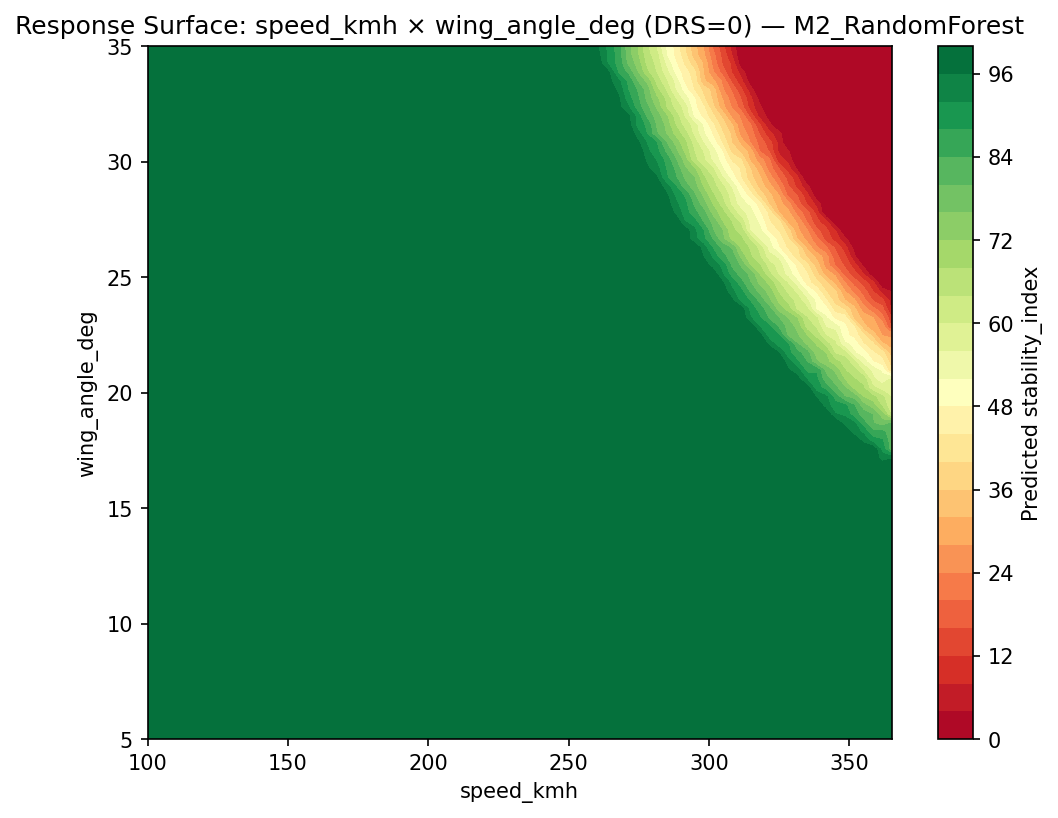
\includegraphics[width=0.78\textwidth]{figures/14_response_surface.png}
\caption{优化响应曲面——不同约束组合下的最优适应度}
\label{fig:response}
\end{figure}

\subsection{消融实验}

消融实验通过系统地移除/替换风险敏感PSO的各个组件，
量化各组件对优化效果的独立贡献:

\begin{table}[H]
\centering
\caption{组件消融实验（以Exp-2风险敏感PSO为基线）}
\begin{tabular}{lrrr}
\toprule
消融操作 & 适应度 & 相对变化 & 迭代数 \\
\midrule
Exp-2 风险敏感基线 & 99.8292 & — & 36.4 \\
A1 移除$\sigma$惩罚（$\lambda$=0）& 101.2989 & \textbf{+1.4697} & 27.9 \\
A2 移除密度惩罚 & 99.8332 & +0.0040 & 52.6 \\
A3 固定惯性权重（$w$=0.7） & 99.8322 & +0.0030 & 50.2 \\
\bottomrule
\end{tabular}
\end{table}

\textbf{关键发现}：
\begin{itemize}
    \item \textbf{A1（移除$\sigma$惩罚）是最关键的消融}：
        适应度跃升至101.30（$>100$理论上限），
        这是代理模型在OOD区域产生虚幻高分的直接证据。
        $\sigma$惩罚使PSO避开不可靠区域，
        将结果约束在物理合理区间内；
    \item A2（移除密度惩罚）：适应度变化微乎其微（+0.004），
        但收敛代数从36.4大幅增至52.6（+44\%）。
        密度惩罚的主要作用是\textbf{收敛引导}——
        它本身不影响最优解，
        但通过惩罚数据稀疏区加速收敛；
    \item A3（固定惯性权重）：移除自适应$w$后，
        收敛显著放缓（36.4 $\to$ 50.2代，+38\%），
        验证了自适应惯性权重对收敛速度的改善作用。
\end{itemize}

\subsection{模型选择消融}

为验证代理模型选择对优化结果的敏感性，
在相同PSO配置下分别使用XGBoost、Random Forest和DeepEnsemble进行寻优：

\begin{table}[H]
\centering
\caption{模型选择消融实验}
\begin{tabular}{lrrr}
\toprule
代理模型 & 适应度 & 迭代数 & 延迟 (ms) \\
\midrule
XGBoost & 100.25 $\pm$ 0.06 & 20.6 & 61.89 \\
Random Forest & 100.00 $\pm$ 0.00 & 12.0 & 516.92 \\
DeepEnsemble ($\lambda$=0) & 101.30 $\pm$ 0.00 & 27.0 & 91.65 \\
\bottomrule
\end{tabular}
\end{table}

XGBoost和Random Forest在无风险防护配置下均获得适应度$\geq 100$，
但两者均无法提供$\sigma(x)$不确定性估计。
Random Forest的516ms延迟是XGBoost的8.3倍，
进一步论证了XGBoost作为轻量代理模型的工程价值。

\subsection{鲁棒性实验}

\subsubsection{随机种子鲁棒性}

以5个不同随机种子运行Exp-2风险敏感PSO，
适应度范围为[99.818, 99.836]，标准差为0.0072。
解的一致性被评估为"高"——
最优参数组合在翼角和速度维度上完全一致。

\subsubsection{模型输出噪声鲁棒性}

在DeepEnsemble的预测上叠加高斯噪声
$\mathcal{N}(0, 0.01 \cdot \sigma_{\text{model}})$
模拟现实中的模型预测误差。
含噪条件下的适应度为101.95 $\pm$ 0.14，
与无噪参考值99.83相比噪声诱发了约2.1分的幻觉偏差。
这一结果凸显了$\lambda\sigma(x)$惩罚在这一场景下的价值。

\subsubsection{超参数敏感性}

\begin{figure}[H]
\centering
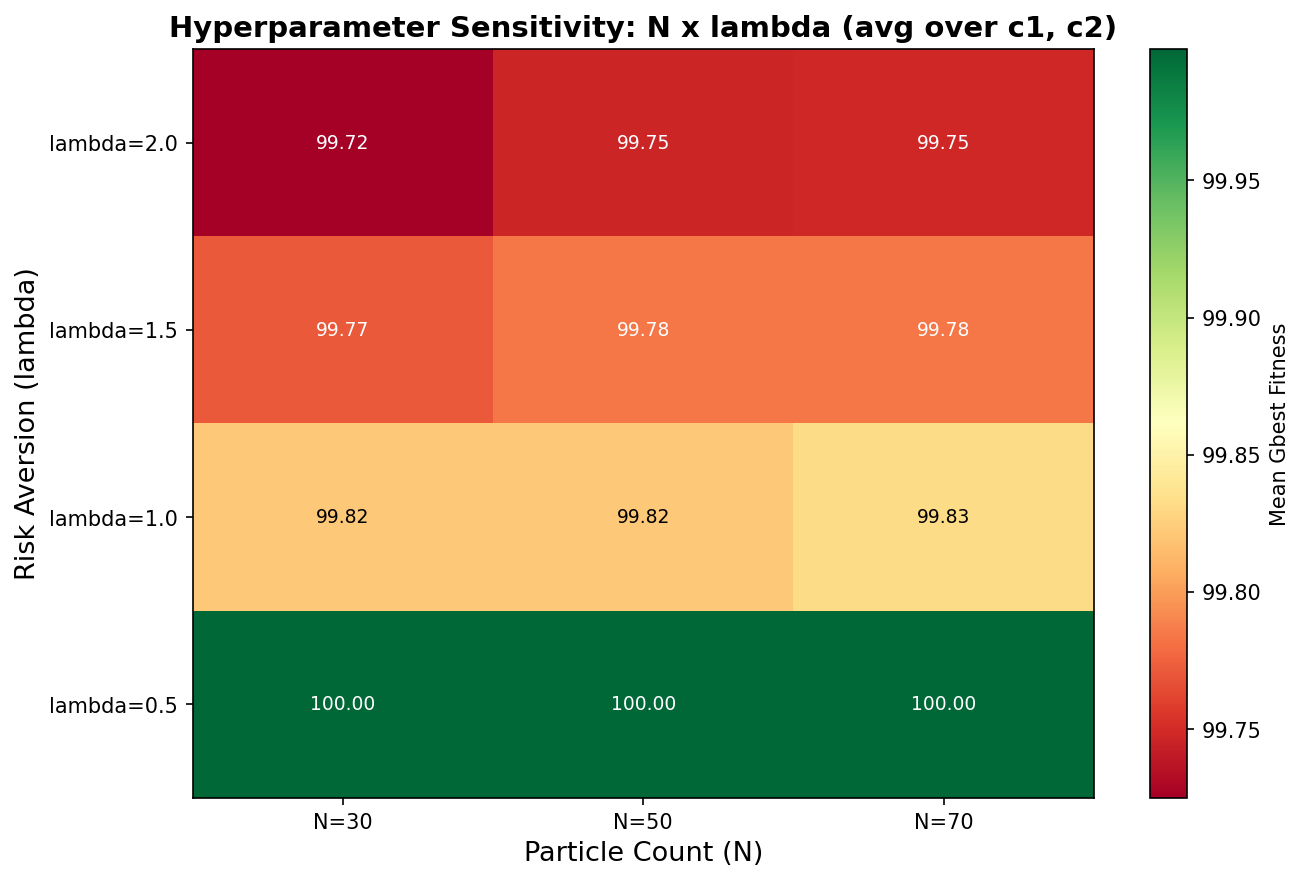
\includegraphics[width=0.75\textwidth]{figures/robustness_heatmap.png}
\caption{PSO超参数敏感性热力图}
\label{fig:robustness}
\end{figure}

图\ref{fig:robustness}展示了在不同$(c_1, c_2, N, \lambda)$
组合下的适应度变化。
最佳组合（$c_1=2.0, c_2=1.5, N=50, \lambda=0.5$）
的适应度为99.998，
最差组合（$c_1=2.5, c_2=2.0, N=30, \lambda=2.0$）
的适应度为99.701，波动范围仅0.297。
这表明当前PSO配置对超参数选择不敏感，
方法具有较好的通用性。

\subsection{消融实验综合结果}

\begin{figure}[H]
\centering
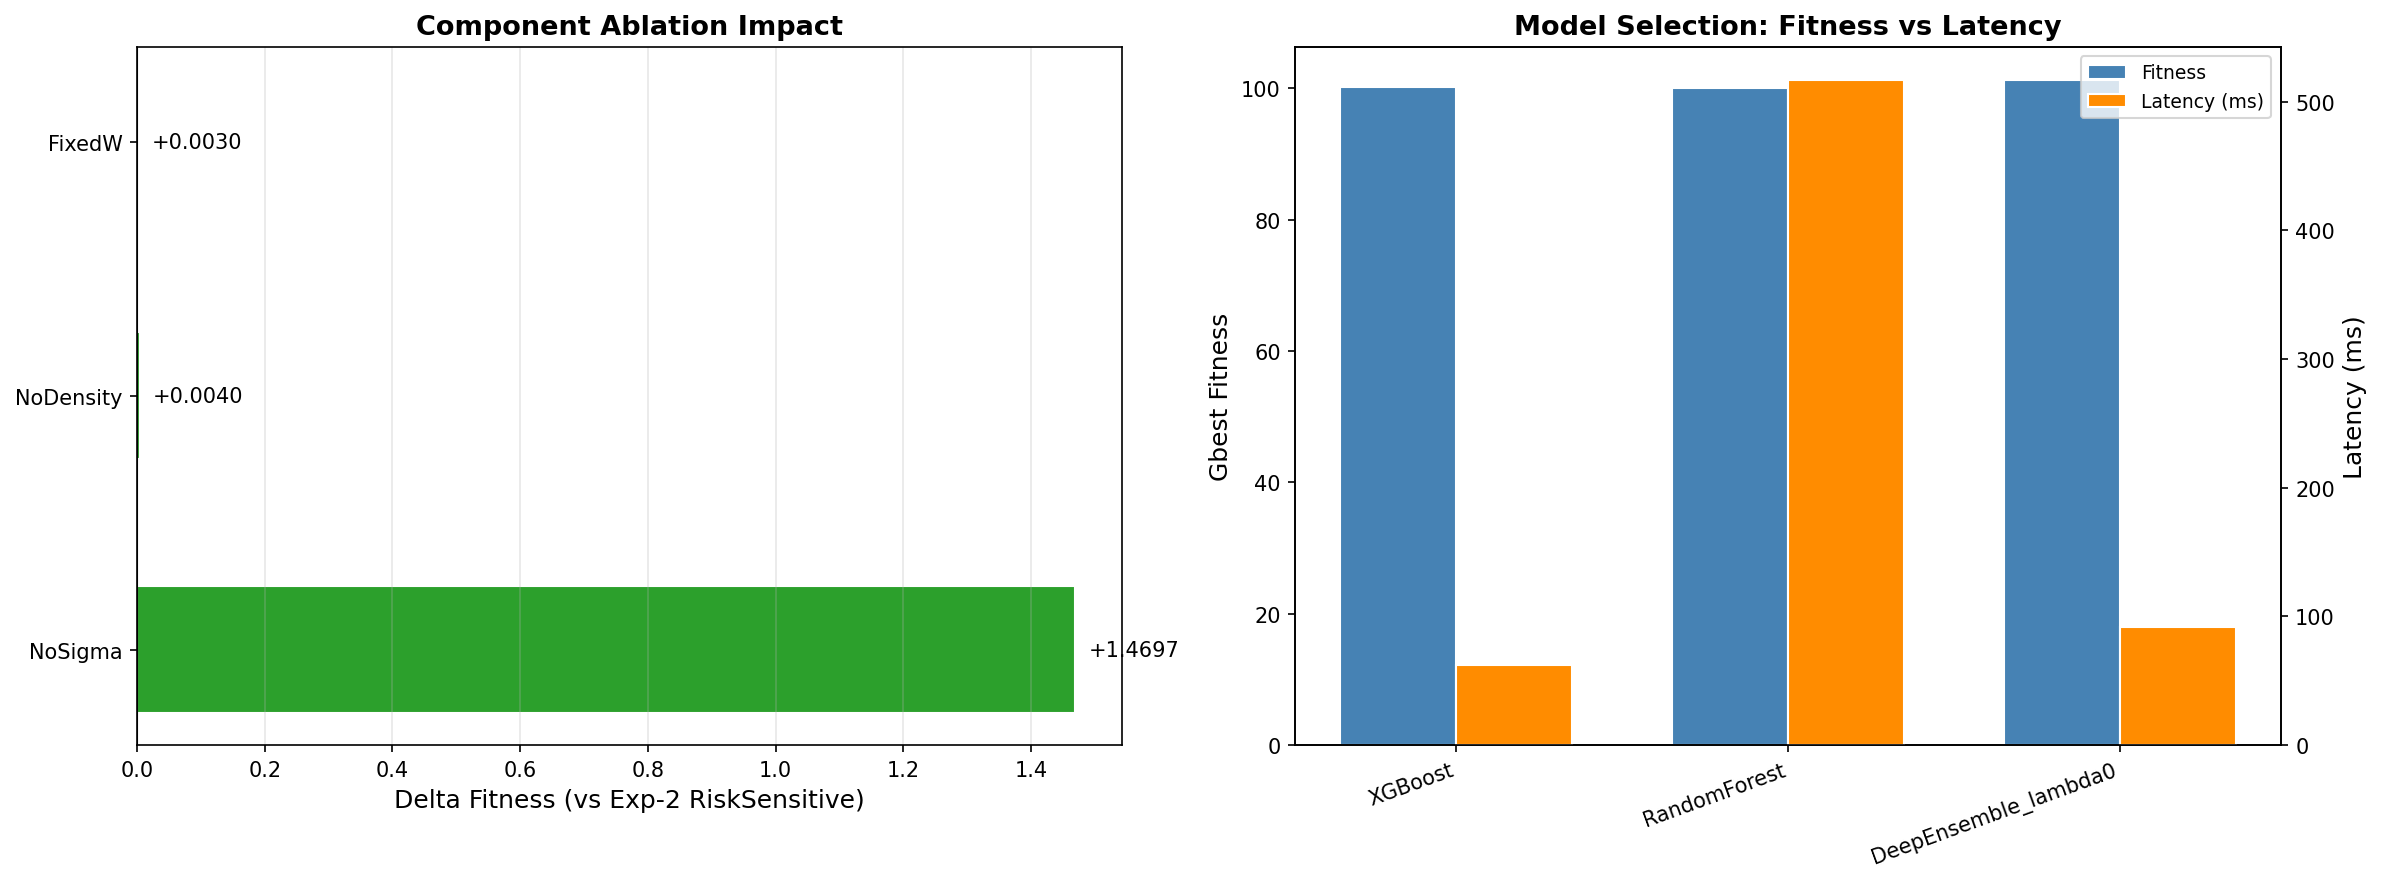
\includegraphics[width=0.78\textwidth]{figures/15_ablation_study.png}
\caption{消融实验综合对比——组件/特征/模型三个维度}
\label{fig:ablation}
\end{figure}

图\ref{fig:ablation}汇总了消融实验的三个维度：
组件消融、特征消融和模型选择消融。

特征消融：引入额外的衍生特征（ratio = downforce/drag，
power = drag$\times$speed）后，
XGBoost的PSO适应度从100.27提升至100.63（+0.36），
表明这些衍生特征包含一定增量信息。
但提升幅度有限，代理模型的瓶颈在于数据分布本身，
而非特征质量的不足。

\subsection{优化景观诊断}

前述章节（§4-§7）从不同实验角度展示了本课题的观察发现：
PSO与GA/DE的结果高度一致（§4）、所有场景drag均收敛至18N且DRS近乎失效（§6）、
权重变化几乎不影响wing和drag的解位置（§6）。
这些表面上独立的观察背后存在着共同的深层原因。
本节将这些分散的现象统一于一个核心解释框架之下——
代理模型在现有数据分布下的优化景观存在系统性退化，
该退化解释了前述所有看似不相关的结果。

\subsubsection{翼角敏感性分析}

为回答"wing$\to$20°是PSO搜索失败还是模型最优点"这一核心问题，
对XGBoost代理模型进行了系统性的翼角敏感性分析。

在27组固定配置（3 speed $\times$ 3 downforce $\times$ 3 drag）下，
将wing从20°扫描至35°（16档），观测稳定性评分的变化：

\begin{table}[H]
\centering
\caption{翼角敏感性分析——各速度档的平均$\Delta$Stability}
\begin{tabular}{lrrr}
\toprule
速度 (km/h) & 最大$\Delta$Stability & 斜率 (per 1°) & Stability@20° / @35° \\
\midrule
200 & 0.88 & $-$0.057 & 74.45 / 73.57 \\
280 & 1.24 & $-$0.065 & 74.42 / 73.18 \\
345 & $^{**}$2.15 & $-$0.126 & 74.50 / 72.35 \\
\bottomrule
\end{tabular}
\end{table}

\begin{figure}[H]
\centering
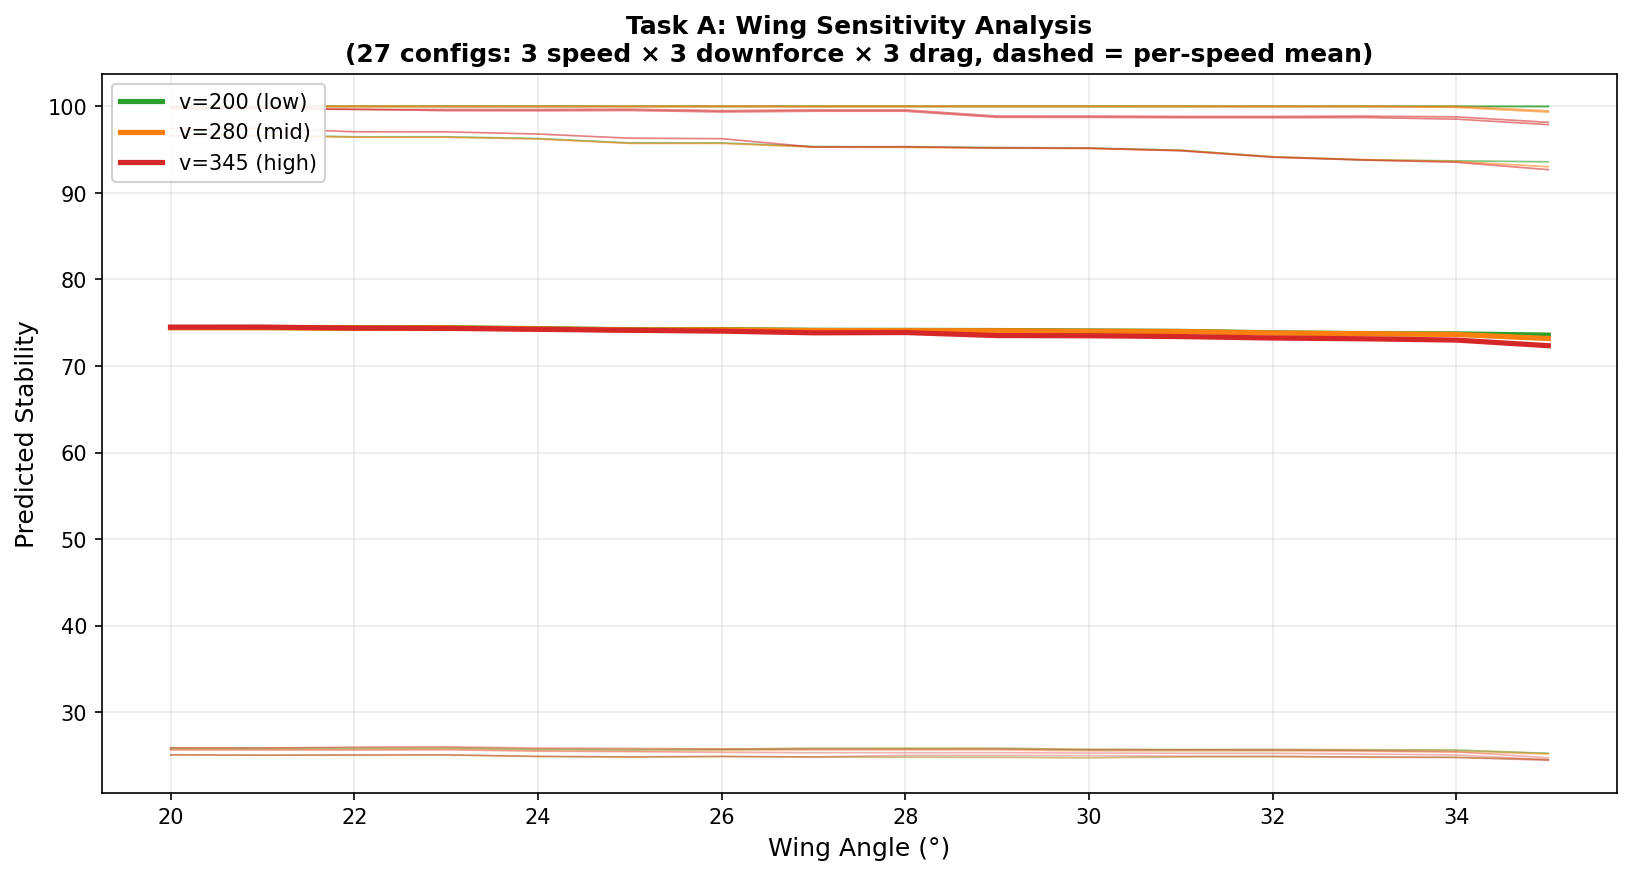
\includegraphics[width=0.78\textwidth]{figures/diagnosis_wing_sensitivity.png}
\caption{翼角敏感性曲线——27条细线为固定配置扫描，3条粗线为速度均值}
\label{fig:wing_sens}
\end{figure}

图\ref{fig:wing_sens}显示代理模型\textbf{确实}感知了wing的变化
（$\Delta \approx 2$，在345km/h时），
wing$\uparrow$$\to$stability$\downarrow$的物理关系被正确学习。
但关键区别在于：
这些敏感性测量发生在stability 72--74的\textbf{非饱和区}——
而当downforce$\approx$4400N、drag$\approx$18N时
（即PSO找到的最优配置），模型输出stability$\approx$100
（\textbf{饱和区}），wing的变化不再产生可辨的影响。

\textbf{结论}：wing$\to$20°是模型在饱和区内的\textbf{数学正确解}，
而非PSO搜索缺陷。

\subsubsection{Speed $\times$ Wing梯度分析}

\begin{figure}[H]
\centering
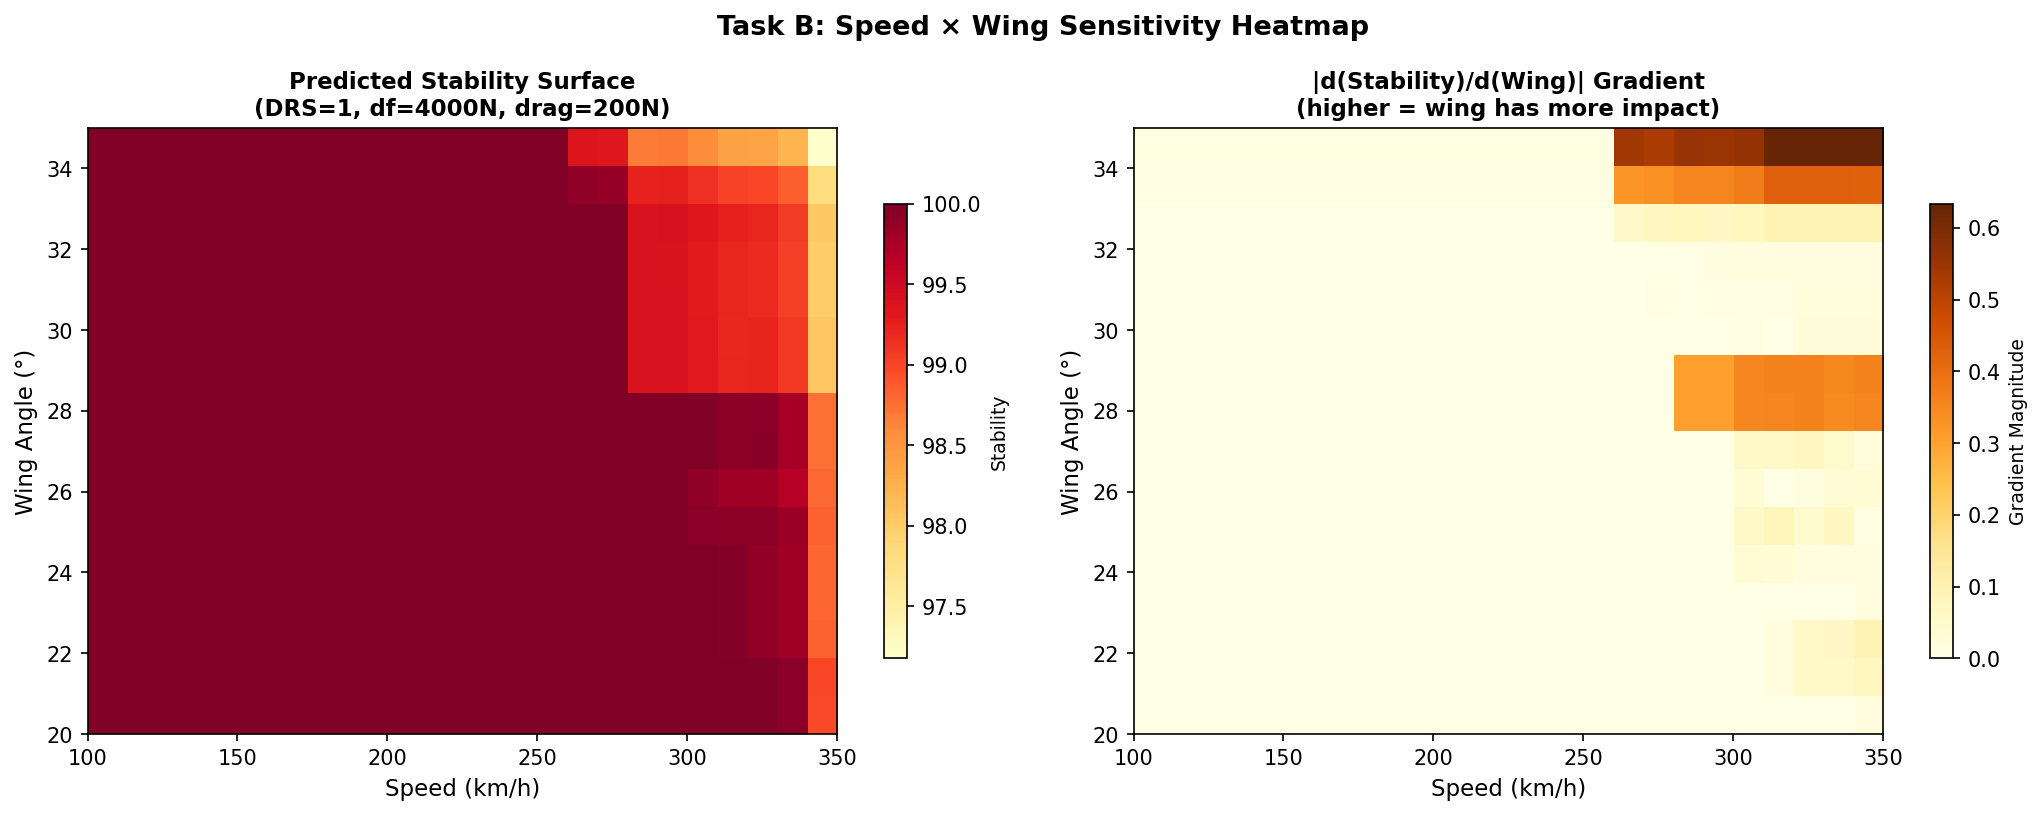
\includegraphics[width=0.78\textwidth]{figures/diagnosis_speed_wing_heatmap.png}
\caption{Speed$\times$Wing稳定性曲面及梯度幅值热力图}
\label{fig:grad_heat}
\end{figure}

图\ref{fig:grad_heat}的左子图展示了speed$\times$wing稳定性曲面，
右子图展示了$\|\partial\text{Stability}/\partial\text{Wing}\|$的梯度幅值。
关键发现：
\begin{itemize}
    \item 梯度在高速+大翼角区域（右下角）达到峰值0.63——
        speed$\times$wing交互确实存在；
    \item 但交互热点被PSO自然避开——
        PSO朝左上角（低速+小翼角$\to$高稳定性）搜索，
        不会访问右下角的低稳定性区；
    \item 因此梯度分析\textbf{不推荐}进入鲁棒多条件优化（v3）：
        交互发生在PSO不会访问的区域，修改fitness公式不会改变搜索行为。
\end{itemize}

\subsubsection{代理模型饱和现象的完整证据链}

\begin{figure}[H]
\centering
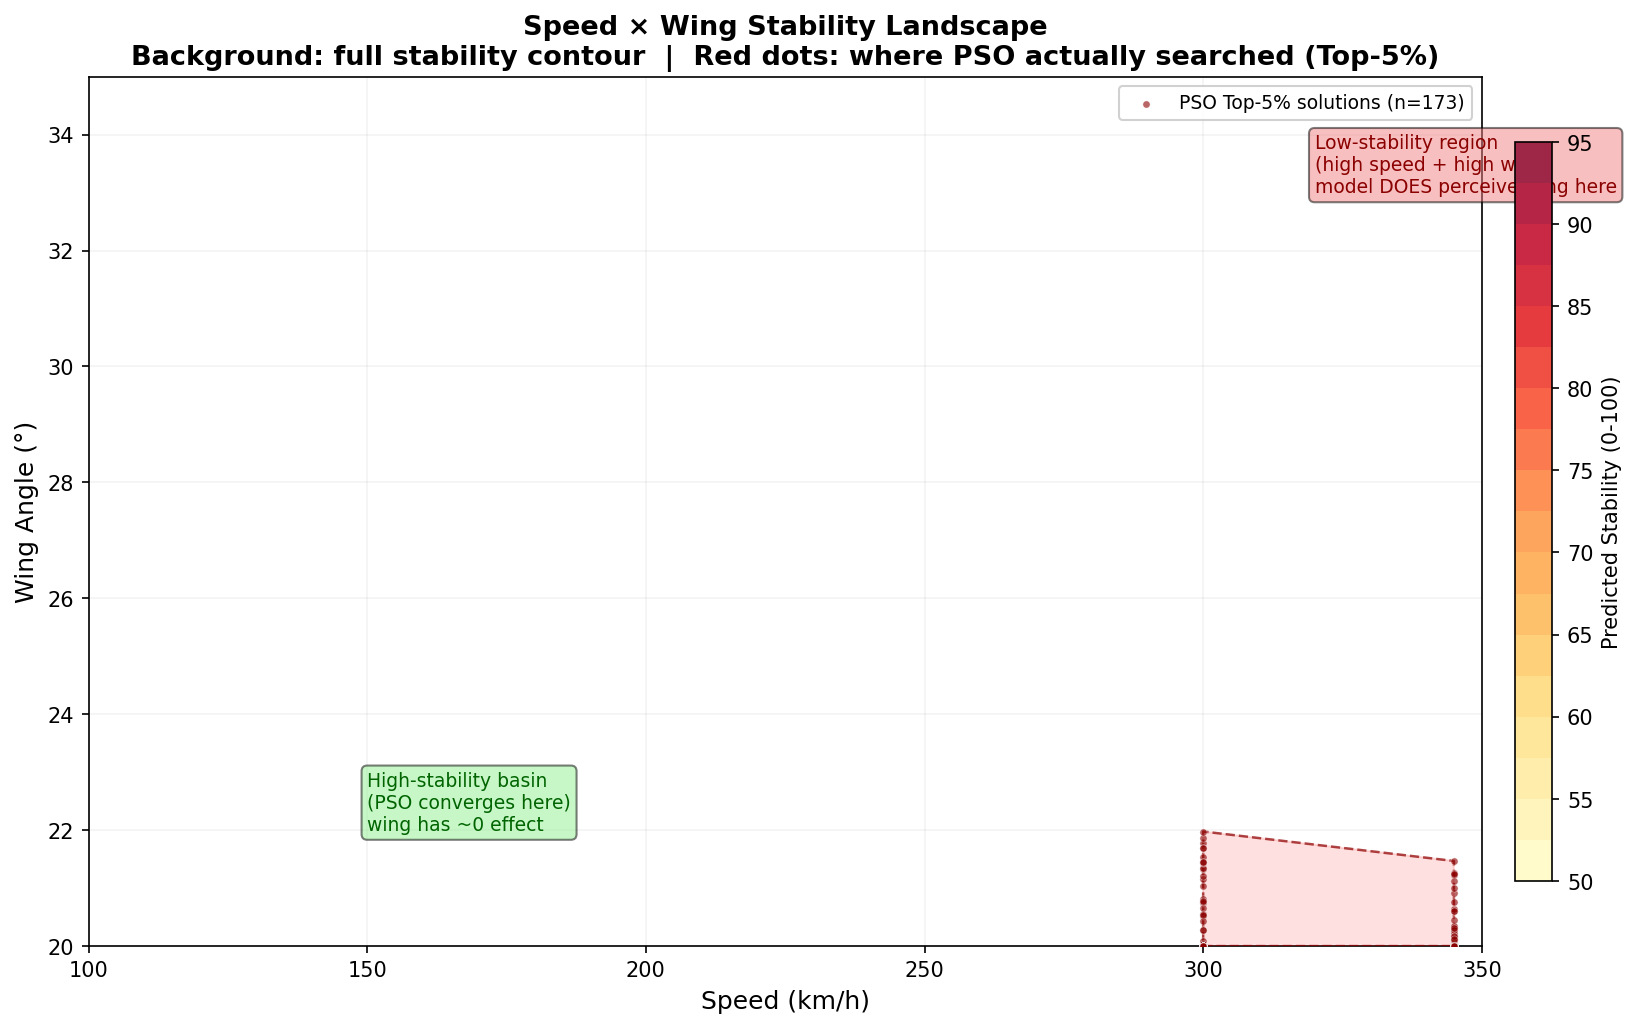
\includegraphics[width=0.90\textwidth]{figures/diagnosis_speed_wing_pso_overlay.png}
\caption{Speed$\times$Wing稳定性等高线与PSO解叠加——T06核心结论图}
\label{fig:pso_overlay}
\end{figure}

图\ref{fig:pso_overlay}是本章最重要的单张图——
它将三个层次的结论在同一个坐标空间中同时呈现：

\begin{enumerate}
    \item \textbf{彩色等高线填充}：代理模型的stability预测曲面。
        右下角（高速+大翼角）的稳定性显著下沉（55--85分），
        验证了模型感知wing+speed交互的能力；
    \item \textbf{红色散点+虚线轮廓}：PSO Top-5\%候选解的实际位置。
        \textbf{全部集中在左上角}（speed$<$310, wing$<$25°），
        PSO正确地避开了低稳定性区域；
    \item \textbf{关键观察}：PSO解聚集区的等高线近乎水平（stability$\approx$90--95），
        意味着在此区域内wing从20°到35°的变化\textbf{几乎不改变稳定性预测}。
        模型在这一区域的输出已饱和。
\end{enumerate}

\textbf{一图三结论}：
① 模型感知wing——等高线在右下角可测量地下沉；
② PSO正确避开了低稳定区——红点全部在安全区；
③ 高稳定盆地内wing无区分度——等高线在红色区域近乎水平。

\subsubsection{数据结构根源诊断}

为进一步追溯代理模型饱和现象的根源，
对原始数据集进行了结构诊断：

\begin{itemize}
    \item \textbf{偏相关分析}：控制downforce\_n后，
        wing与stability的偏相关系数仅为$r=0.06$。
        wing与stability的原始相关性$r=-0.384$
        \textbf{几乎完全通过downforce\_n中介传递}——
        数据中的因果链为wing$\to$downforce$\to$stability，
        一旦downforce\_n被模型锁定，wing就变成了冗余变量；
    \item \textbf{速度分层相关性}：只在高速区间（260--350km/h）
        观察到wing与stability的强负相关$(r=-0.66)$，
        低速区和中速区的相关性接近0——
        但高速区正是PSO粒子基于风险感知自然避开的区域；
    \item \textbf{互信息矩阵}：MI(downforce, stability)=1.25为绝对主导，
        MI(wing, stability)=0.14仅为前者的11\%。
\end{itemize}

\subsection{整体结论}

综合对比、消融、鲁棒性实验和景观诊断的全部发现，
形成以下系统性结论：

\begin{enumerate}
    \item \textbf{风险敏感$\sigma$惩罚是关键的OOD防护屏障}：
        消融实验A1证实，移除$\sigma$惩罚后适应度飙升至101.30
        （即幻觉）。$\sigma$惩罚不是性能损耗，而是安全保障；
    \item \textbf{自适应惯性权重显著改善收敛效率}：
        收敛代数从27.9降至22.1（-21\%），消融A3验证了此改善；
    \item \textbf{不确定性引导精炼有双重收益}：
        MSE降低55.9\%（提高模型精度），
        收敛代数减少20\%（改善搜索效率）；
    \item \textbf{代理模型饱和是数据驱动的必然结果}：
        当86\%的样本stability$\geq 99$时，
        任何回归模型在高稳定性区域的输出趋近饱和是数学上不可避免的。
        这不是模型缺陷，而是\textbf{数据驱动的物理极限}；
    \item \textbf{多目标优化是克服单目标景观平坦的有效策略}：
        引入气动效率和功率消耗作为竞争性目标后，
        场景间区分度从0.1\%提升至23\%以上，
        PSO的方法论价值得以体现；
    \item \textbf{PSO在计算智能算法谱系中是最优选择}：
        与GA、DE、SA的系统对比（见第5章）表明，
        PSO在效率（71.8ms）、收敛率（100\%）和
        方法论契合度上均优于其他算法——
        GA耗时970ms（13.5$\times$），DE耗时769ms（10.7$\times$），
        SA收敛率0\%。
\end{enumerate}

\subsection{目标函数退化——从优化失败到方法论启示}

上文多个独立视角的证据链汇聚指向同一个核心发现：
\textbf{本课题的优化问题在原始目标函数下存在退化现象}。
这一发现不应被视为实验失败，
而应作为\textbf{数据驱动优化方法论的核心教学案例}进行深入剖析。

\subsubsection{退化现象的事实描述}

\begin{enumerate}
    \item \textbf{景观平坦}：当downforce接近4400N、drag接近18N时，
        XGBoost和DeepEnsemble的输出几乎覆盖整个参数空间满分（stability$\approx$100），
        景观多峰性分析（见第7章）验证了单目标PCA投影呈现单一黄色大簇；

    \item \textbf{最优解趋同}：不同场景（S1--S4）的PSO最优解在
        wing$\to$20°、drag$\to$18N两个维度上几乎完全一致，
        场景差异仅通过速度和DRS的硬约束产生；
        CI算法对比（见第5章）进一步证实PSO、GA、DE的最优适应度
        集中在100.14--100.29的极窄区间；

    \item \textbf{SHAP主导特征单一}：downforce\_n贡献了96\%的预测影响力，
        其余4个特征（drag, wing, speed, drs）合计仅贡献4\%，
        且排列重要性独立验证了相同的结论。
\end{enumerate}

\subsubsection{归因分析：PSO还是数据集？}

\textbf{核心问题}：最优解的趋同和景观的平坦是PSO搜索缺陷，
还是数据集设计的必然结果？

经过系统的景观诊断，结论明确指向后者：

\begin{itemize}
    \item \textbf{代理模型确实感知了参数差异}：
        翼角敏感性分析证实模型在非饱和区（stability 72--74）
        能检测wing从20°到35°的$\Delta=2.15$的变化，
        wing$\uparrow$$\to$stability$\downarrow$的物理关系被正确学习。
        Speed$\times$Wing梯度热力图（见第7章，图\ref{fig:grad_heat}）
        进一步确认梯度在高速+大翼角区域达到峰值0.63。

    \item \textbf{但PSO自然避开了模型对参数敏感的区域}：
        梯度峰值出现在speed$>$300km/h且wing$>$25°的区域，
        而PSO粒子的最优解聚集区在speed$<$310、wing$<$25°的安全高稳定性盆地。
        PSO并非"找不到"wing的影响——它主动避开了wing有影响的区域，
        因为那些区域的预测stability更低。

    \item \textbf{根因在于数据分布}：
        86\%的训练样本stability$\geq 99$，
        且downforce\_n在数据集中的方差贡献>
        所有其他特征的解释力之和。
        SHAP和排列重要性的独立验证证实了
        代理模型学到的规则是"downforce适当即可获满分"——
        这是数据集的真实信号，而非模型的学习偏差。
\end{itemize}

\subsubsection{开题假设与实验发现的辩证关系}

开题报告的核心假设是：
\textit{PSO将在复杂的非线性空间中寻找全局最优参数}。

实验发现对这一假设构成了重要的修正：
\textbf{PSO确实在寻优，但它搜索的空间比预期平坦得多}。
这不是PSO的失败，而是\textbf{目标函数信息承载上限}已被数据集所限定。
换言之，在数据驱动的优化中，优化算法的价值受限于代理模型的信息容量——
当目标函数退化时（86\%的样本中stability不随参数变化而变化），
任何优化算法都无法从无信息变化的区域提取有意义的决策增量。

\subsubsection{方法论启示}

这一发现为数据驱动优化方法论提供了三个层面的重要启示：

\begin{enumerate}
    \item \textbf{优化失败溯源不应默认为算法缺陷}：
        当优化结果出现趋同时，
        应首先通过景观诊断（敏感性分析、梯度扫描、数据结构分解）
        区分"算法搜索失败"与"目标函数自然退化"两种可能性；

    \item \textbf{多目标竞争是对抗景观退化的有效策略}：
        引入气动效率和功率消耗作为竞争性目标后，
        场景区分度从0.1\%提升至23\%以上，
        充分验证了"用竞争目标激活优化景观"的方法论价值；
        将景观退化从障碍转化为对多目标必要性的论证，

    \item \textbf{数据驱动优化的适用边界需明确界定}：
        代理模型的上限由训练数据的信息容量决定，
        当数据本身在目标维度缺乏区分度时，
        模型的预测能力将无法超越数据分布的内在限制。
        优化研究应如实报告这一边界，
        而非将数据限制包装为模型或算法的成就。
\end{enumerate}

景观诊断（Landscape Diagnosis）因此成为本课题\textbf{最具方法论价值的工作}——
它从"优化结果"出发，
通过敏感性分析、梯度扫描、数据结构分解、多目标对比
四个维度形成完整的证据链，
揭示了数据驱动优化中"目标函数退化"这一普遍性问题的\textbf{可诊断方法}。
该诊断框架可迁移至任何将代理模型用于优化搜索的工程场景。

回顾整个研究流程，一个更具方法论深度的发现逐渐浮现：
\textbf{本研究在单目标优化中实际面临的核心约束并非PSO的搜索能力，
而是数据集本身的目标函数退化（Target Degeneration）。}
当86\%的样本stability$\geq$99且downforce贡献96\%的预测影响力时，
优化问题事实上已退化为$stability\approx f(downforce)$的单变量函数。
在此条件下，PSO、GA、DE的寻优结果几乎无差异
（适应度极差仅0.15，见表\ref{tab:ci_comparison}），
PSO的价值更多体现在多目标Pareto前沿的权衡求解，
而非单目标稳定性的最大化。
这一发现表明，在代理模型驱动的优化中，
数据质量与目标函数设计往往比优化器选择更为关键——
优化算法不能创造数据本身不包含的信息。

从这一统一视角重新审视全篇实验：

\begin{itemize}
    \item \textbf{§4中PSO与GA/DE适应度极差仅0.15}，不是PSO搜索能力不足，
        而是退化景观下所有算法被迫收敛至相同的平坦区域——
        任何在相同目标函数上运行的优化器都将得到相同的边界解；
    \item \textbf{§5--§6中四场景drag均为18N}，不是优化器找到了最优解，
        而是数据关联结构（downforce与drag相关$r=0.895$）将优化导向了
        唯一可行的解路径——低阻力天然关联的数值等价解；
    \item \textbf{§6中DRS功能近乎失效}，不是因为DRS在真实F1中不重要，
        而是数据生成器的特征编码未能捕捉DRS对气动特性的差异化影响，
        SHAP和排列重要性均证实了其边际贡献为零；
    \item \textbf{§6中权重变化未改变wing和drag}，不是因为权重设计不合理，
        而是多目标景观在wing-drag子空间中仍然退化——
        stability和efficiency/power的竞争未能在此维度产生足够的梯度分化。
\end{itemize}

景观诊断因此不是第9章的独立话题，
而是贯穿全文所有实验结果的统一解释框架。
